\subsection{Tau Reconstruction and Identification}\label{sec:tauID}

The challenge in identifying hadronically decaying taus is discriminating against generic quark and gluon QCD jets 
which are produced with a cross--section several orders of magnitude larger. CMS has developed several algorithms to 
reconstruct and identify
hadronically decaying taus based on Particle Flow (PF) objects. For this analysis, the tau POG 
recommended Hadron Plus Strips algorithm (HPS) is used. HPS makes use of PF jets as 
inputs to an algorithm that uses strips of clustered electromagnetic particles to reconstruct neutral pions. The 
electromagnetic strips (``neutral pions'') are combined with the charged hadrons within the PFJets to attempt to 
reconstruct the main tau decay modes outlined in Table~\ref{table:taumodes}.

\begin{table}[ht][H]
  \caption{Reconstructed Tau Decay Modes}
  \centering{
  \begin{tabular}{| c |}
  \hline\hline
        HPS Tau Decay Modes \\ [0.5ex] \hline
        Single Charged Hadron + Zero Strip \\
        Single Charged Hadron + One Strip \\
        Single Charged Hadron + Two Strips \\
        Two Charged Hadrons \\
        Three Hadrons \\
  \hline
  \hline
  \end{tabular}
  }
  \label{table:taumodes} % is used to refer this table in the text
\end{table}

The single hadron plus zero strips decay mode attempts to reconstruct $\tau \to \nu\pi^{\pm}$ decays or $\tau \to 
\nu\pi^{\pm}\pi^{0}$ decays where the neutral pion has very low energy. The single hadron plus one or two 
electromagnetic strips attempts to reconstruct tau decays that produce neutral pions where the resulting neutral pion 
decays produce collinear photons. Similarly, the single hadron plus two strips mode attempts to reconstruct taus that 
decay via e.g. $\tau \to \nu\pi^{\pm}\pi^{0}$ where the neutral pion decays to well-separated photons resulting in two 
electromagnetic strips. The three hadrons decay mode attempts to reconstruct tau decays that occur with three charged pions (``3-prongs"). Although it is possible to recover signal in the two hadron decay mode (in the case of one of the
three prongs being misidentified), this mode is not considered as its inclusion reduces discrimination performance and 
hurts the limit. 
In all cases, electromagnetic strips are 
required to have $E_{T} > 1$ GeV/c. Additionally,
the particle flow charged hadrons are required to be compatible with a common 
vertex and have a net charge of $|q|=1$.

In order to enforce the isolation requirement on the reconstructed tau, a region of size R = 0.5 around the tau decay  direction is defined. Any PF candidates not used for the reconstruction of electromagnetic strips and charged 
hadrons not involved in the reconstruction of the tau decay modes are used to calculate isolation. The ``Tight'', ``Medium", and/or ``Loose" 3-hits isolation working points are used as recommended by the tau POG. 

Pileup can be a confounding problem in calculating isolation, so corrections for accidentally including particles from the wrong PV in the isolation calculation are applied. It has been empirically determined that the total energy for neutral hadrons and photons coming from pileup is on average equal to about one half of the total energy of charged hadrons from the PV. The correction for this, known as the $\delta\beta$ correction, manifests itself as an extra term in the numerator of the isolation calculation, Equation \ref{eq:iso}. It is applied by subtracting off one half of the \pt sum of charged hadrons in the event \textit{not} originating from the chosen PV. Unless otherwise stated, $\delta\beta$ corrections are applied to every isolation used in this analysis.
%The ``very loose'' working point requires no isolation PF charged hadrons with $p_{T}>1.5$ GeV/c and no 
%isolation PF gamma candidates with $E_{T}>2.0$ GeV.

In order to discriminate against muons, HPS taus are required to pass the lepton rejection 
discriminator which requires the lead track of the tau not be associated with a global muon signature. In order to 
discriminate against electrons, HPS taus are required to pass a MVA discriminator which uses the amount of HCAL energy 
associated to the tau with respect to the measured momentum of the track (H/p). Additionally, the MVA discriminator 
considers the amount of electromagnetic energy in a narrow strip around the leading track with respect to the total 
electromagnetic energy of the tau. Finally, HPS taus must not reside in the ECAL cracks. 
In all channels, the identification and isolation used follows the Tau POG recommended criteria.
The exact discriminator names and working points for each channel are listed and described in their respective sections.




\subsubsection{Efficiency of Tau Identification discriminators} \label{sec:tauIDeff}
The efficiency of the $\tau_{h}$ ID discriminators used in the analysis are studied using $Z^{\prime}_{SSM}$ samples with $m(Z^{\prime}) = 2000$ GeV. For this purpose, we require the reconstructed $\tau_{h}$ to have $p_{T} >$ 45 GeV and pseudorapidity $|\eta| < 2.1$. Further, a reconstructed $\tau_{h}$ is matched to generator-level tau with $\Delta R(\tau_{reco},\tau_{gen}) < 0.3$. The efficiency of the Decay Mode Finding (DMF) discriminator  ``DecayModeFinding'' is found to be relatively flat at $\sim 80$\% as shown in Figure ~\ref{fig:DMF}. The individual efficiencies of anti-muon , anti-electron and isolation discriminators, relative to the DMF criterion, are shown in Figures ~\ref{fig:ML3}--~\ref{fig:TIso}. The overall efficiency of the $\tau_{h}$ ID selection used in this analysis is $\sim 55$\%. We use the POG-recommended VLoose working point of the anti-electron MVA5 discriminator as the tighter working points have poor performance (i.e. low efficiency which is also not ``flat" vs. $p_{T}$). The relative flatness of the $\tau_{h}$ identification efficiency with $p_{T}$ will also facilitate the use of $Z\rightarrow\tau\tau$ events as a "standard candle" for comparison with signal. 

\begin{figure}[tbh!]
    \centering
    \begin{tabular}{cc}
      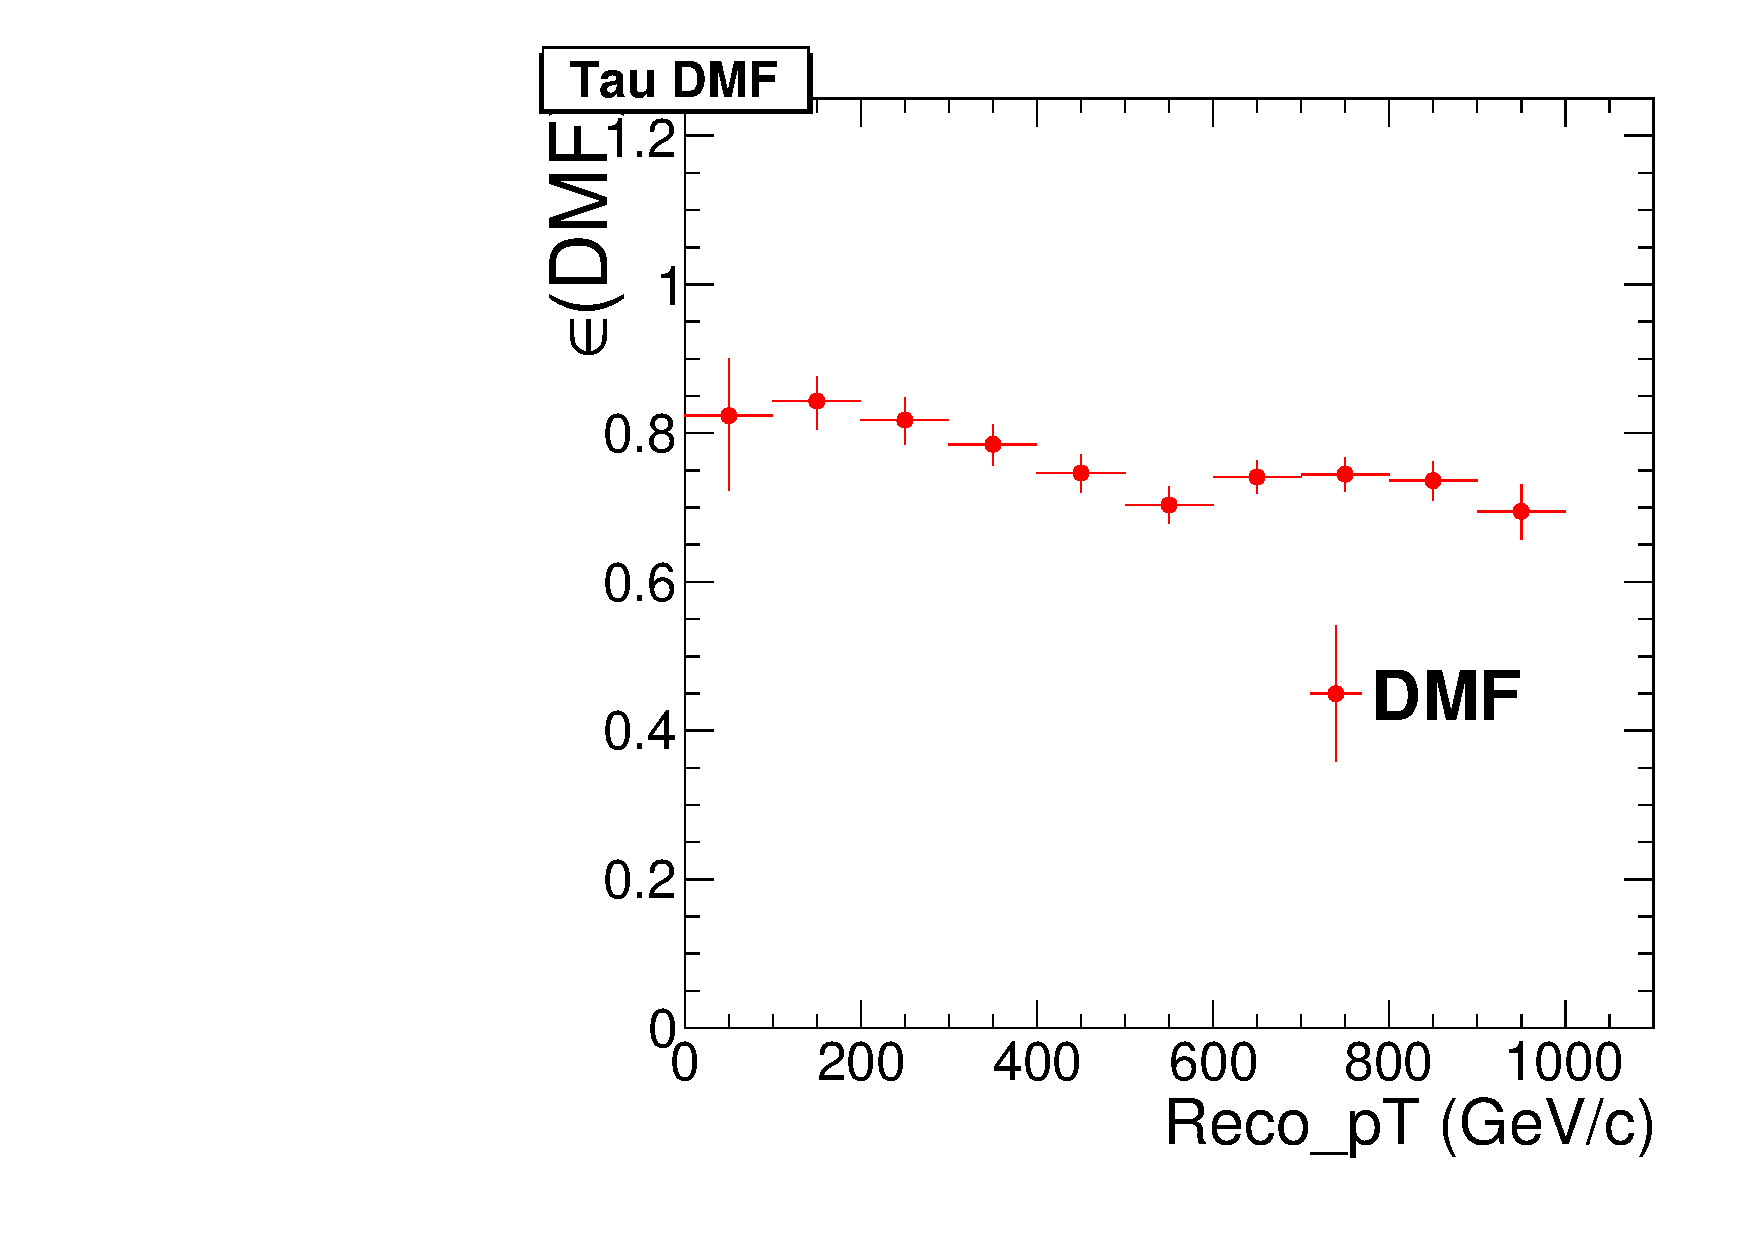
\includegraphics[width=0.30\textwidth]{figures/DMF_4_29_16.pdf}
      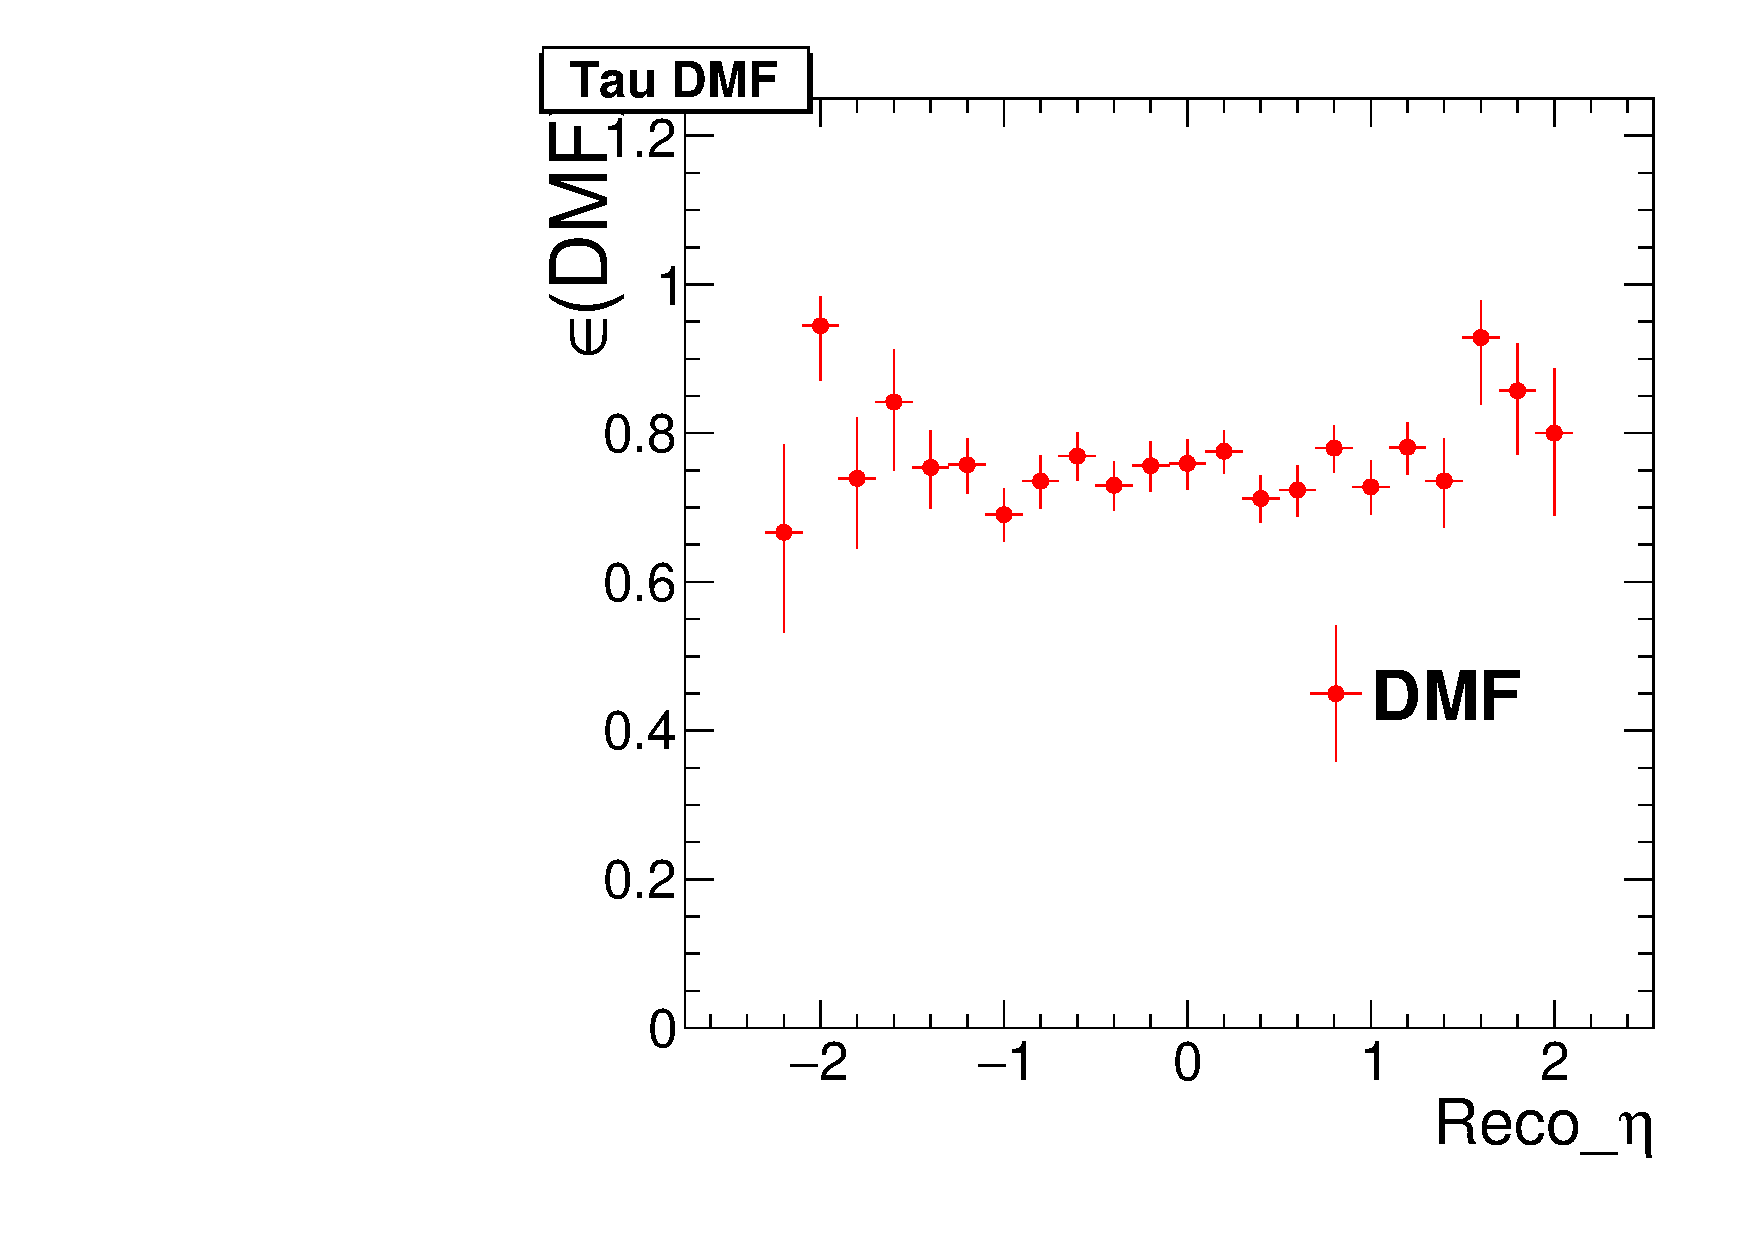
\includegraphics[width=0.30\textwidth]{figures/DMF_eta_4_29_16.pdf}
       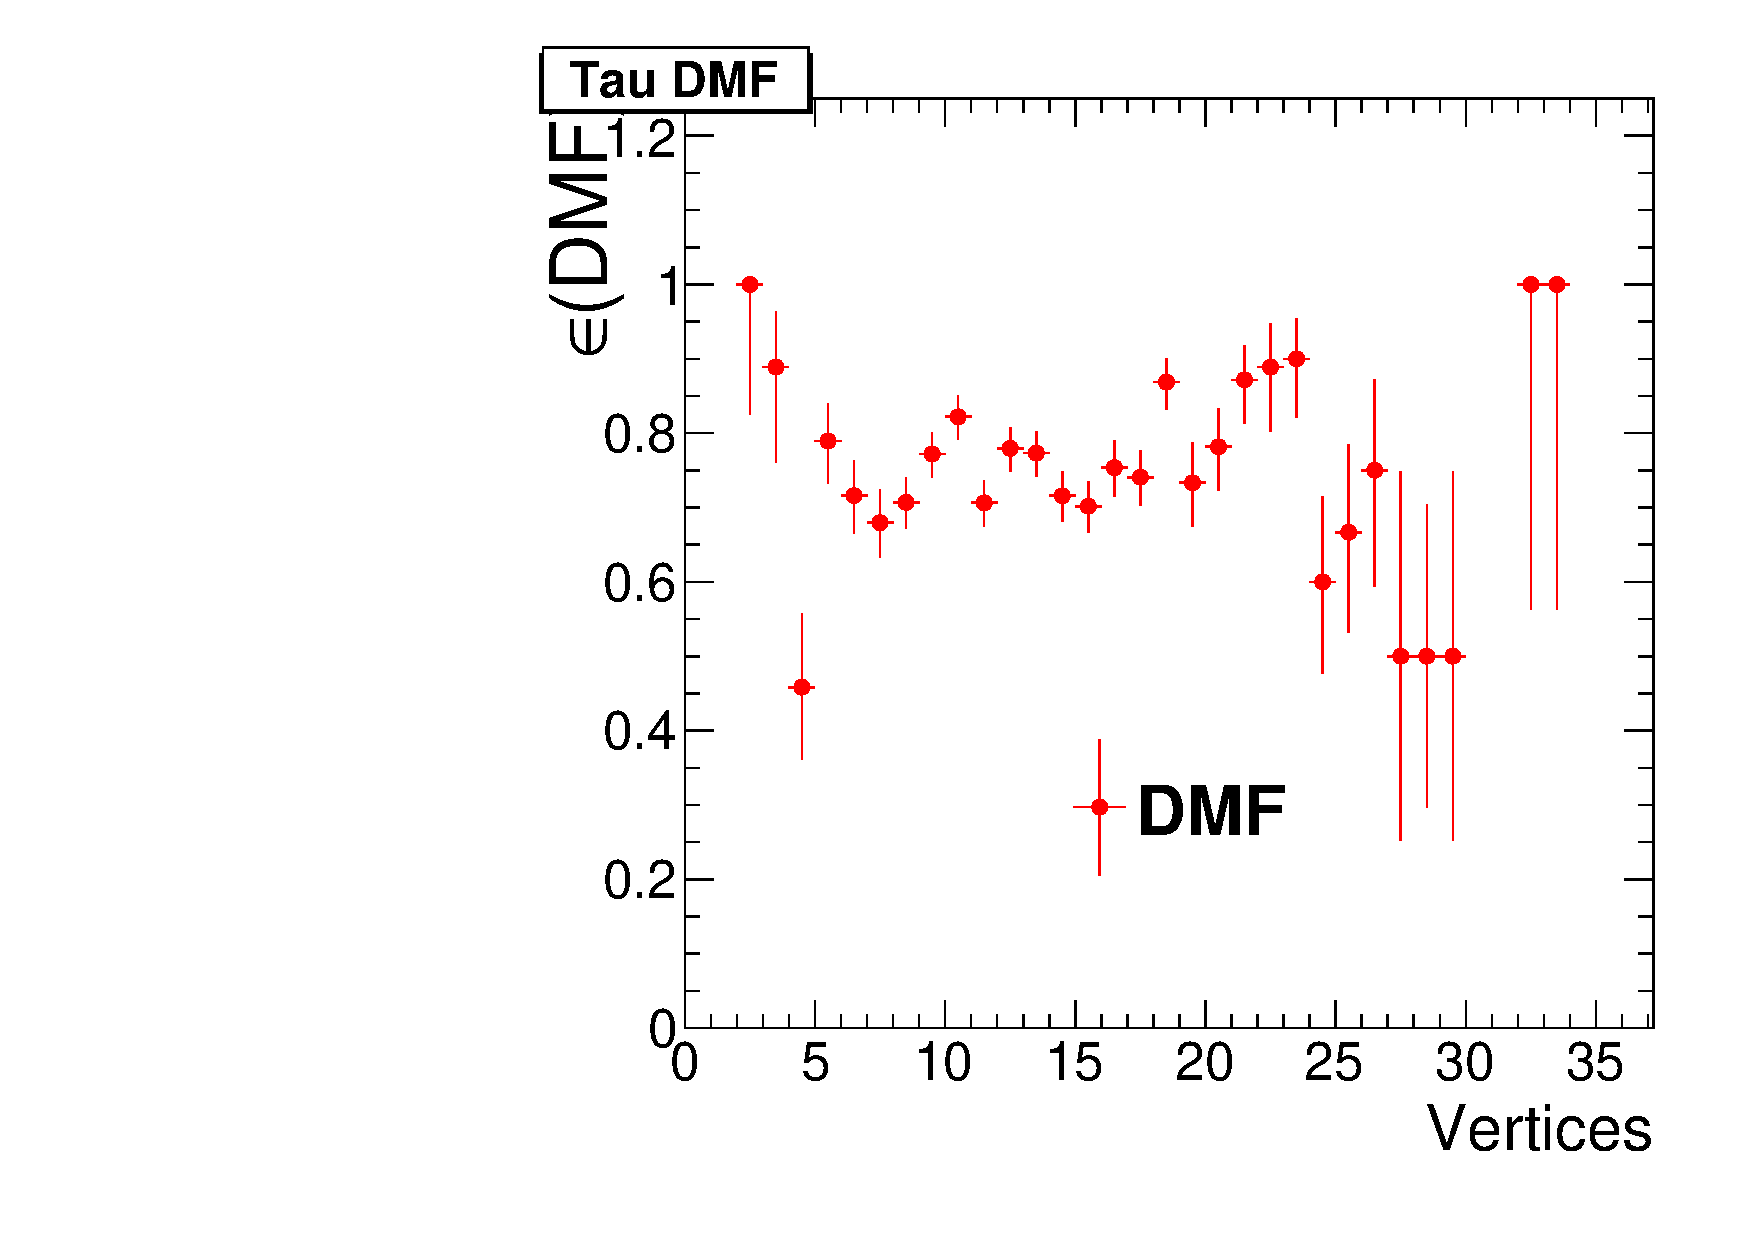
\includegraphics[width=0.30\textwidth]{figures/DMF_nvtx_4_29_16.pdf}
    \end{tabular}
    \caption{Decay Mode Finding efficiency as function of $p_{T}$, $\eta$, and number of vertices of generator-level taus }
    \label{fig:DMF}
  \end{figure}
 
\begin{figure}[tbh!]
    \centering
    \begin{tabular}{cc}
      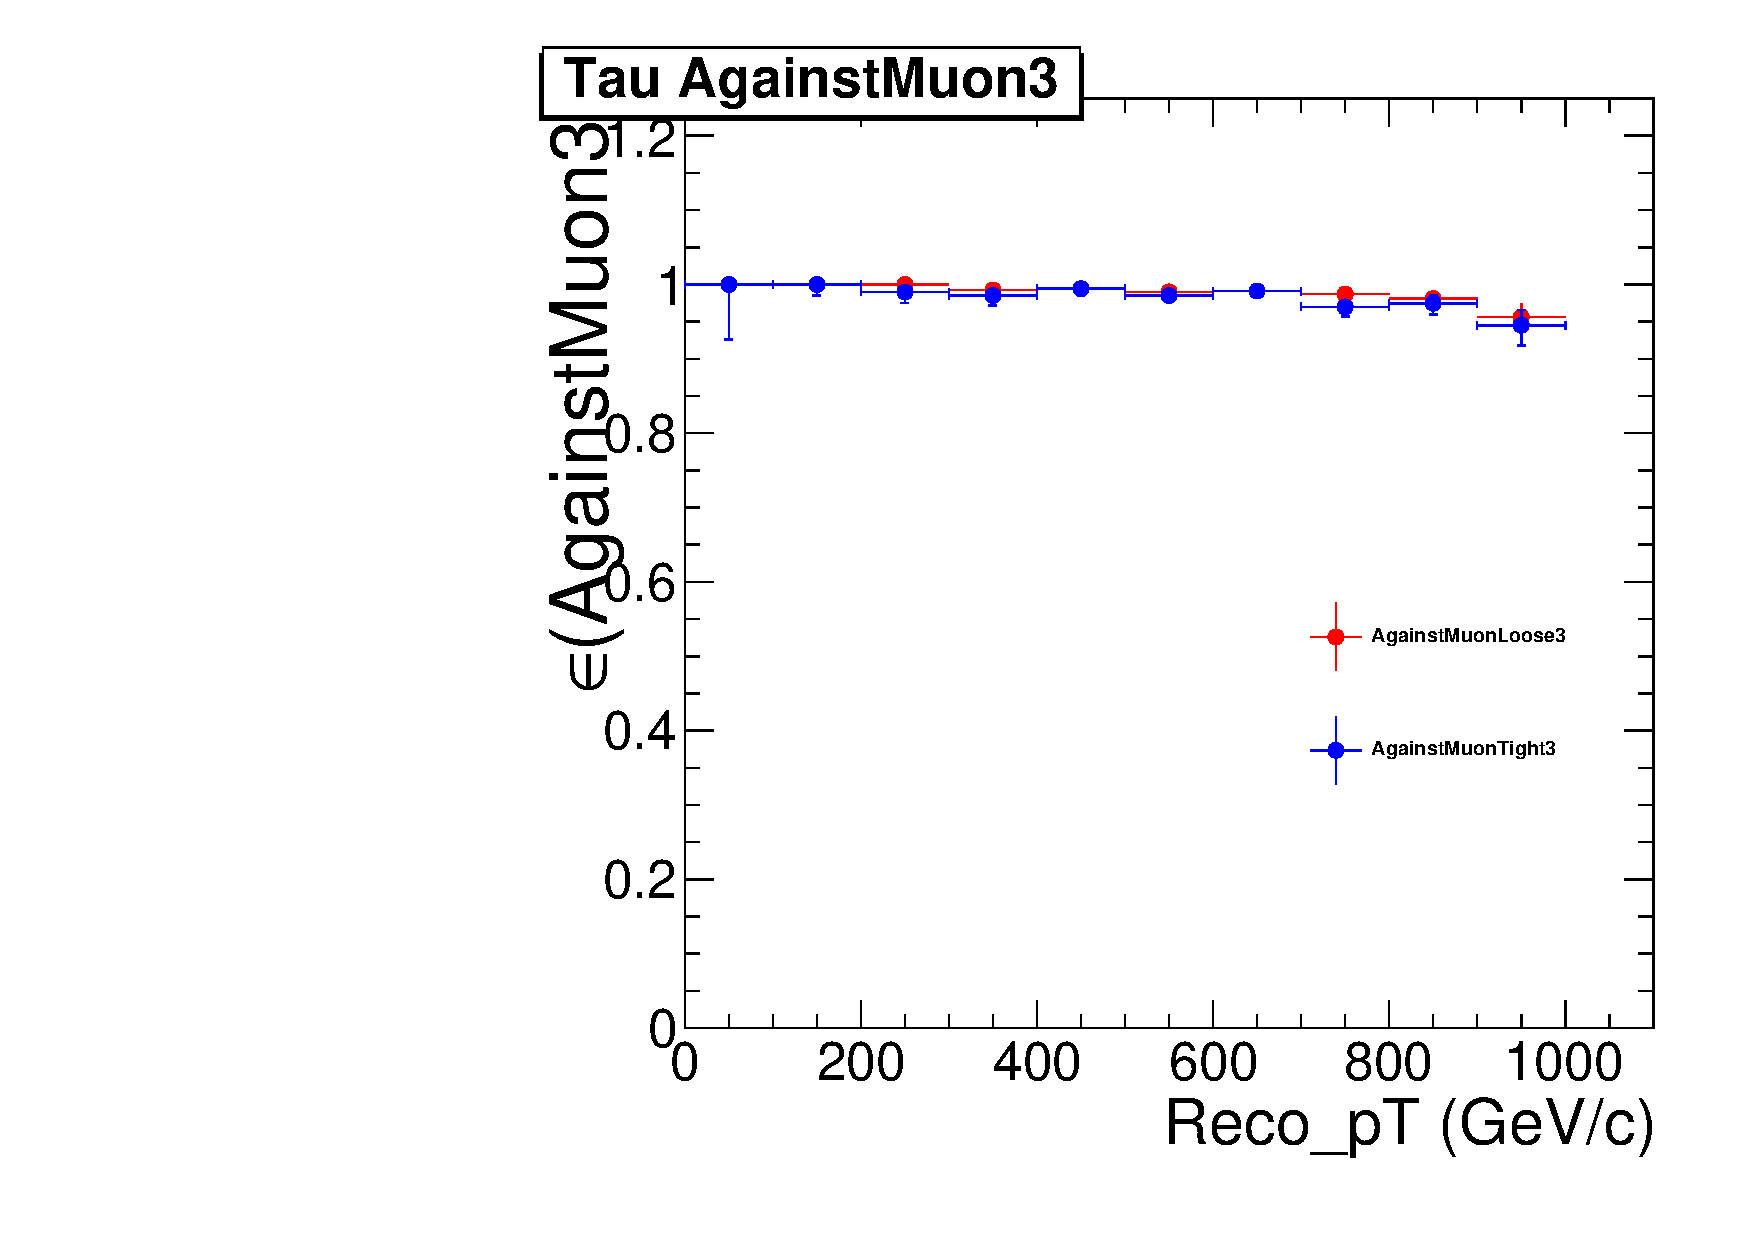
\includegraphics[width=0.30\textwidth]{figures/AgainstMuon_4_29_16.pdf}
      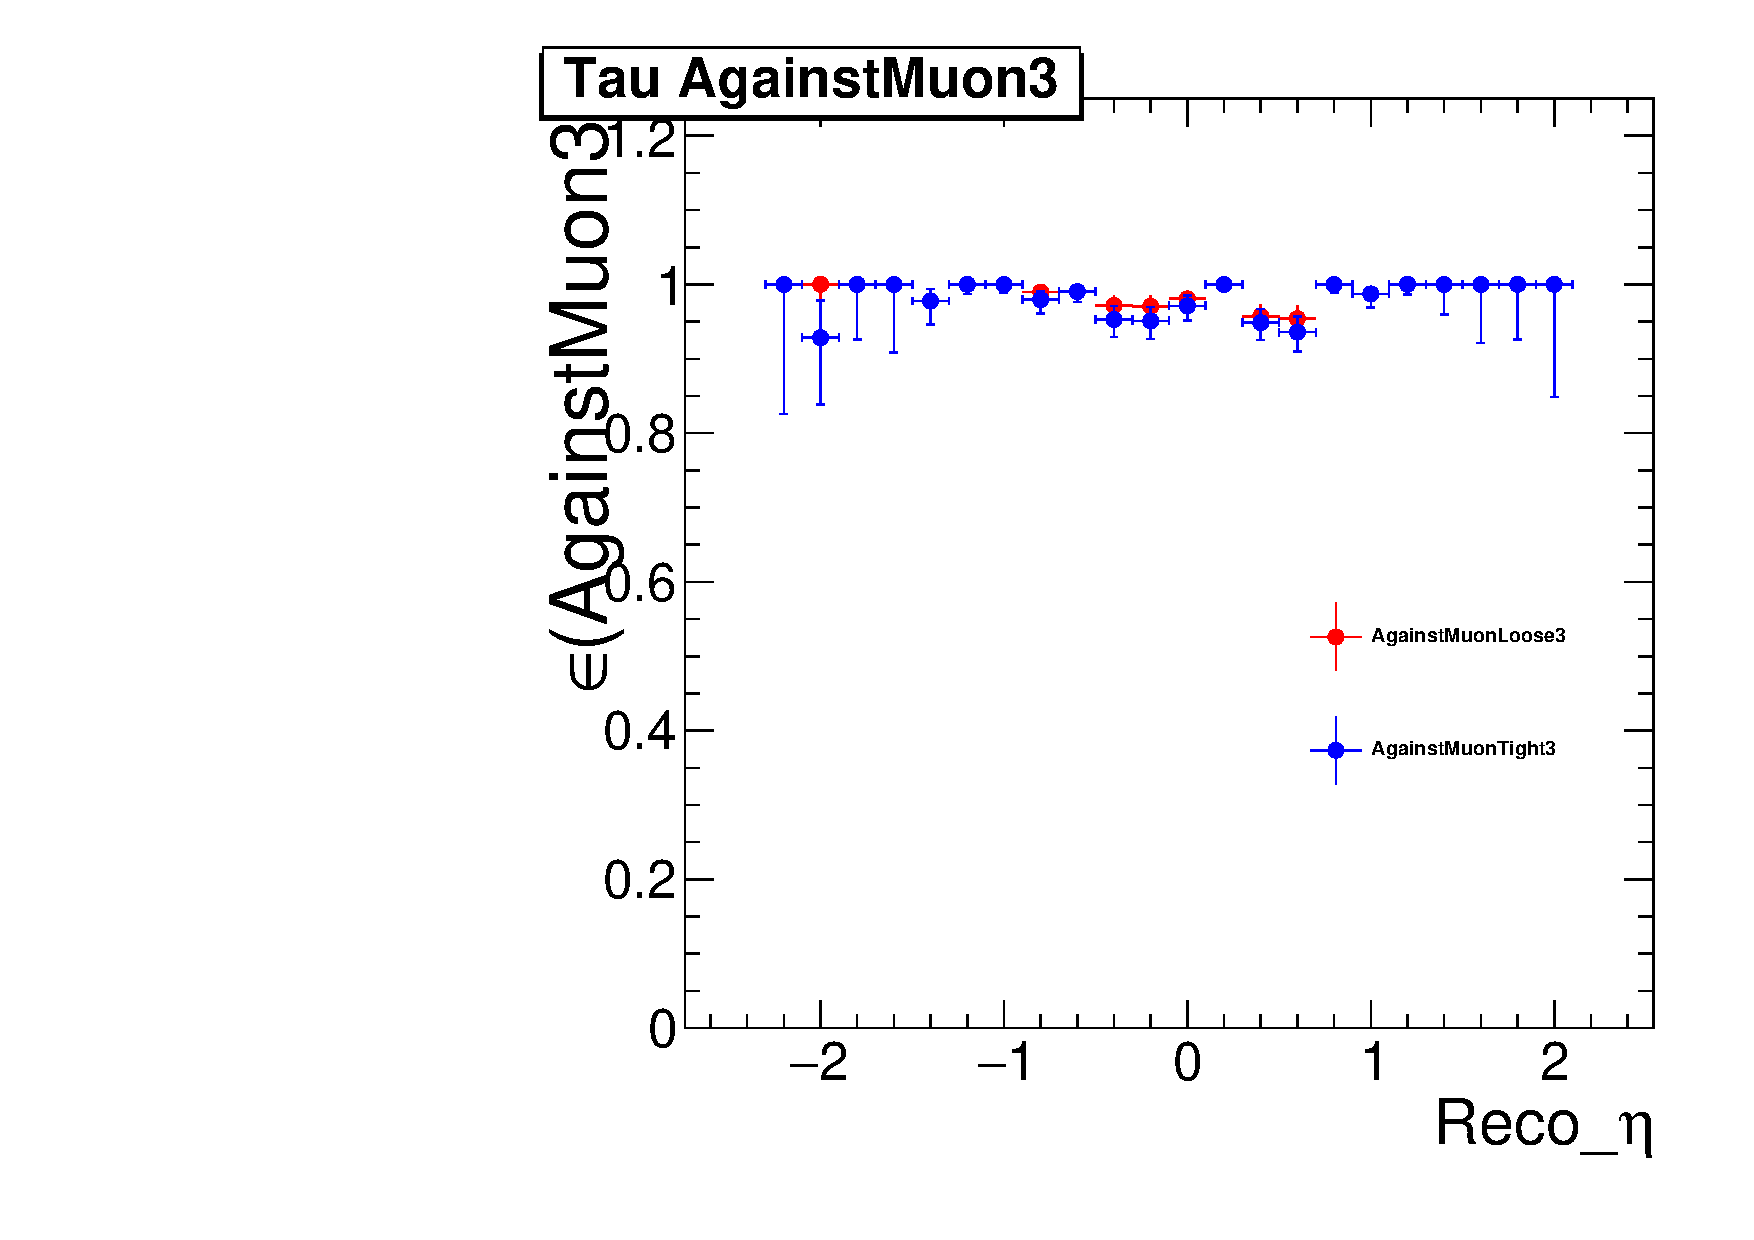
\includegraphics[width=0.30\textwidth]{figures/AgainstMuon_eta_4_29_16.pdf}
       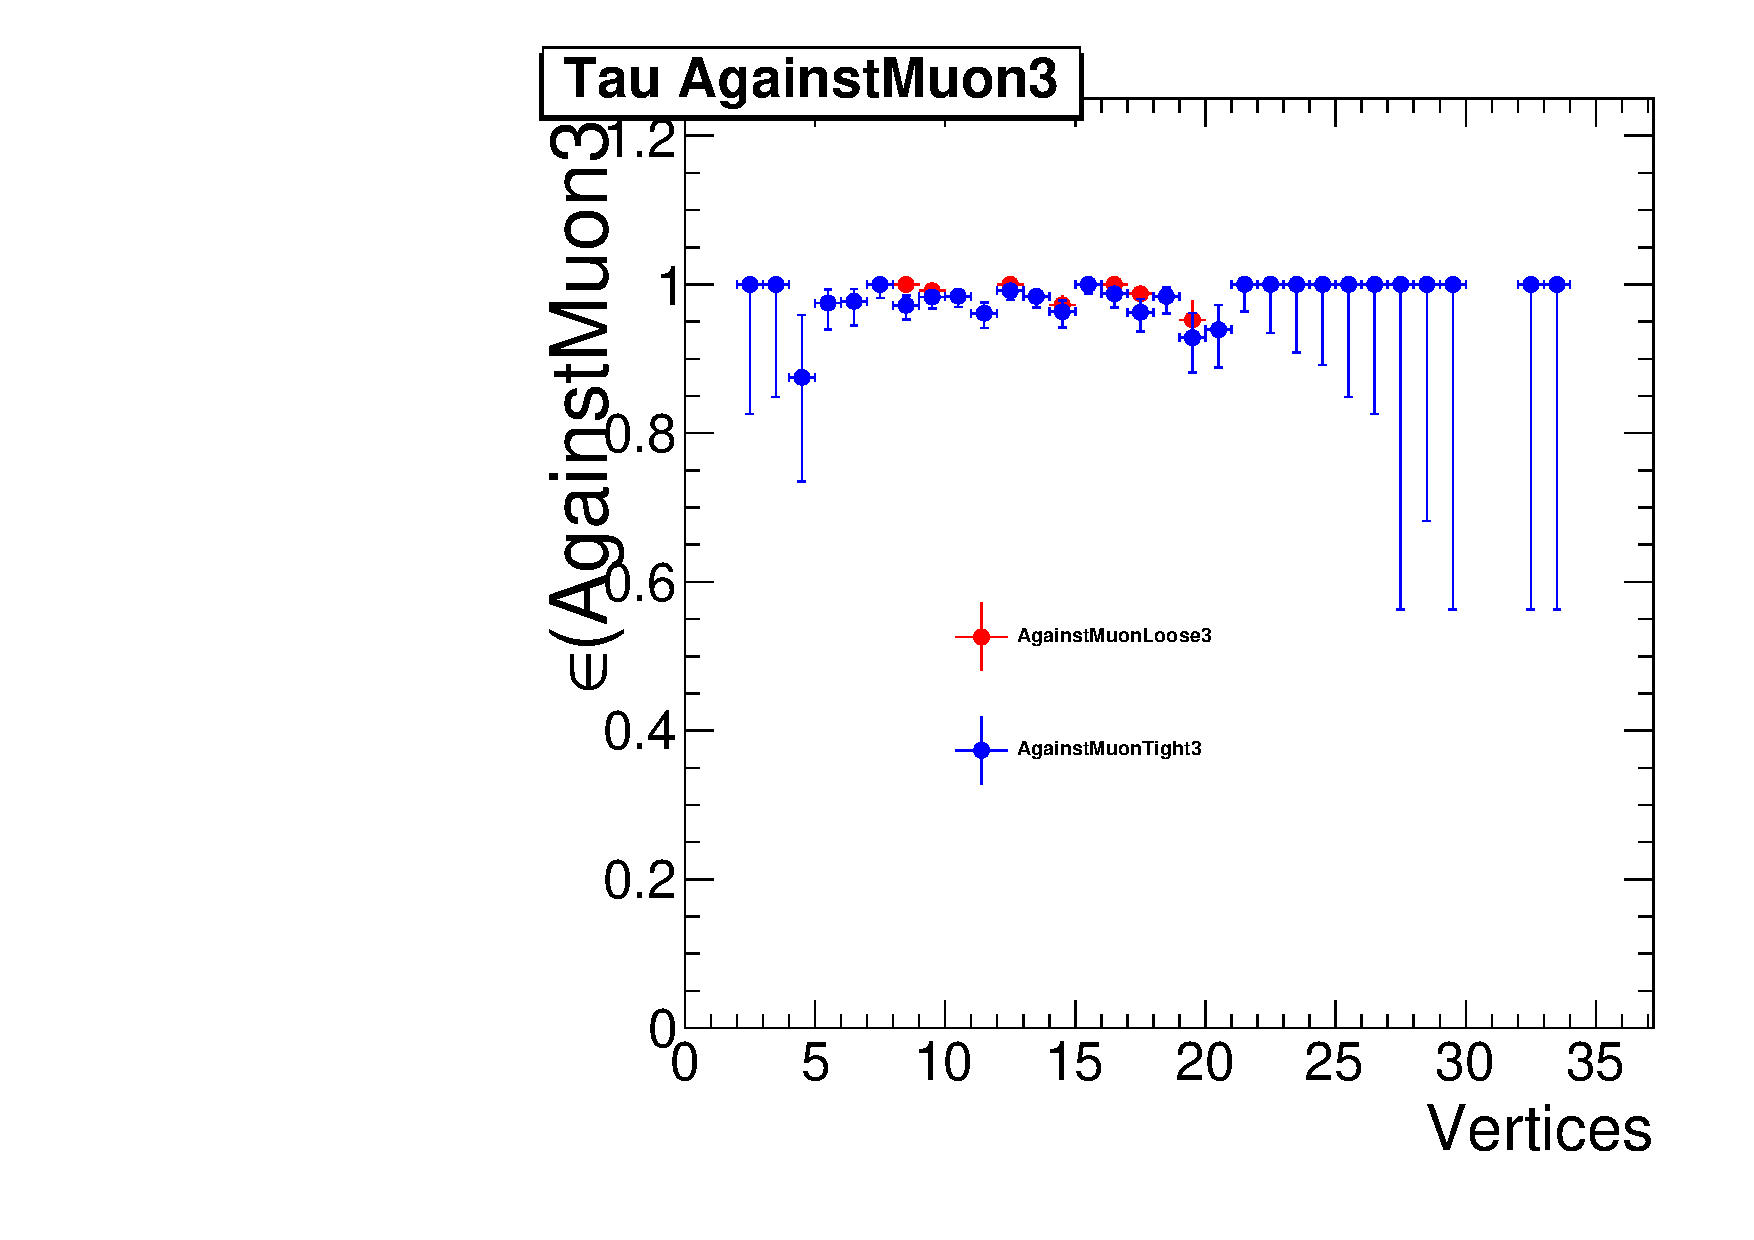
\includegraphics[width=0.30\textwidth]{figures/AgainstMuon_nvtx_4_29_16.pdf}
    \end{tabular}
    \caption{Efficiency of anti-muon discriminator (Loose3) as function of $p_{T}$, $\eta$, and number of vertices of generator-level taus }
    \label{fig:ML3}
  \end{figure}


\begin{figure}[tbh!]
    \centering
    \begin{tabular}{cc}
      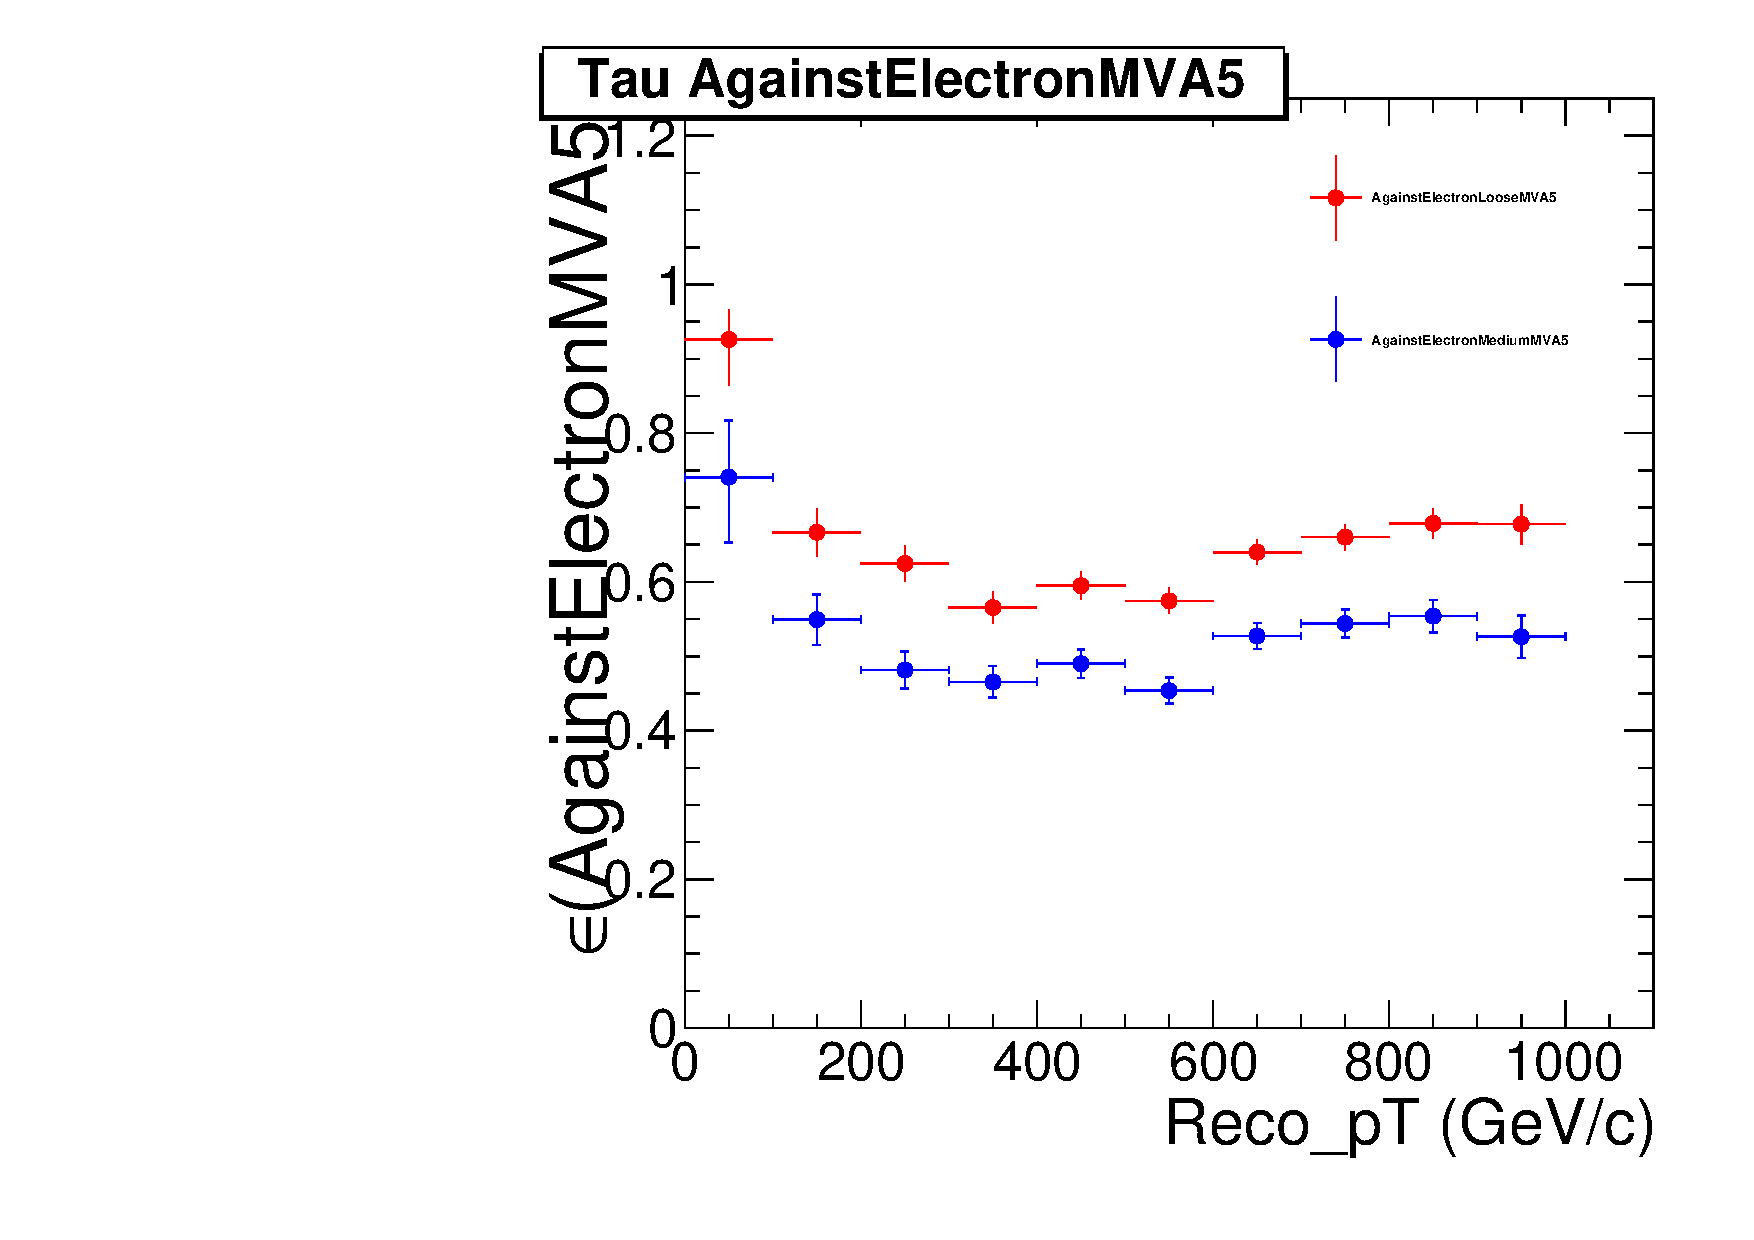
\includegraphics[width=0.50\textwidth]{figures/AgainstElectron_4_29_16.pdf}
      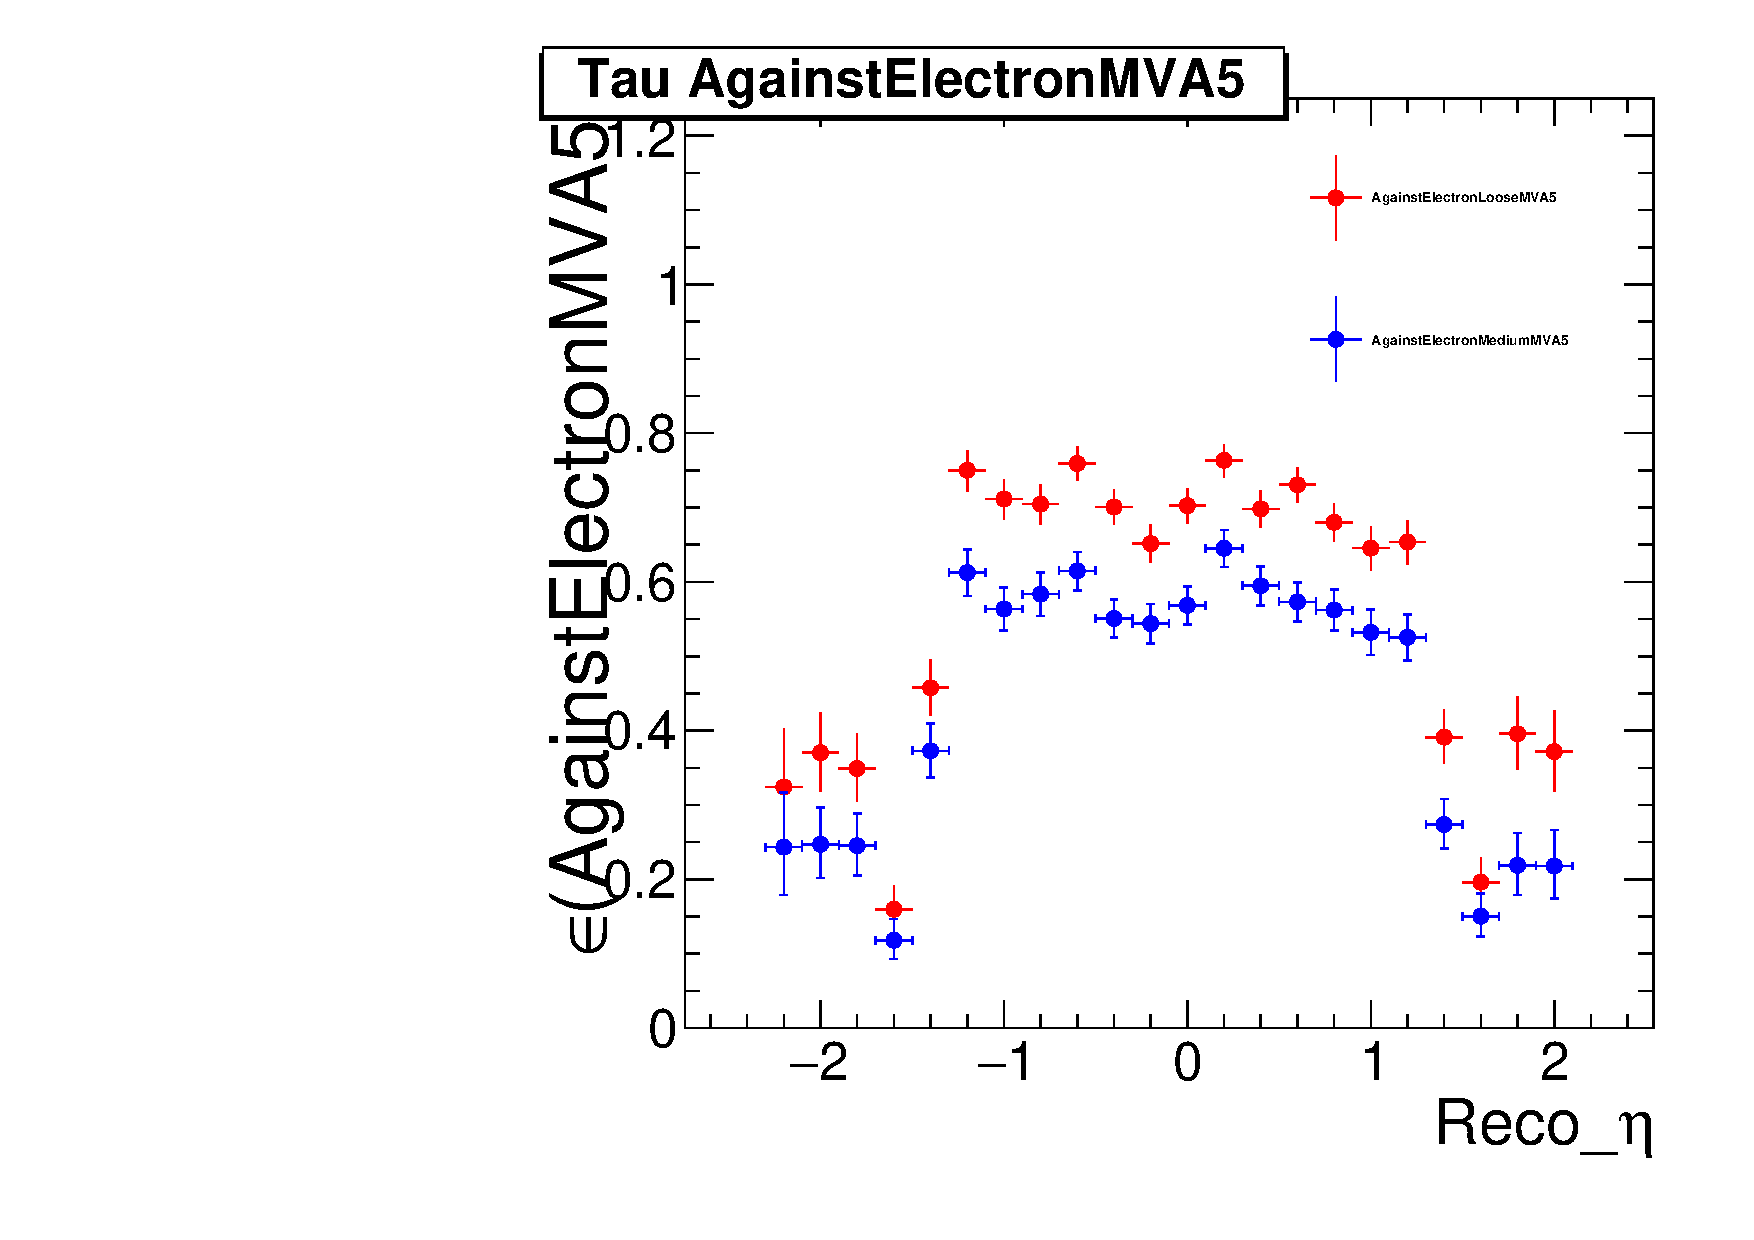
\includegraphics[width=0.50\textwidth]{figures/AgainstElectron_eta_4_29_16.pdf}
       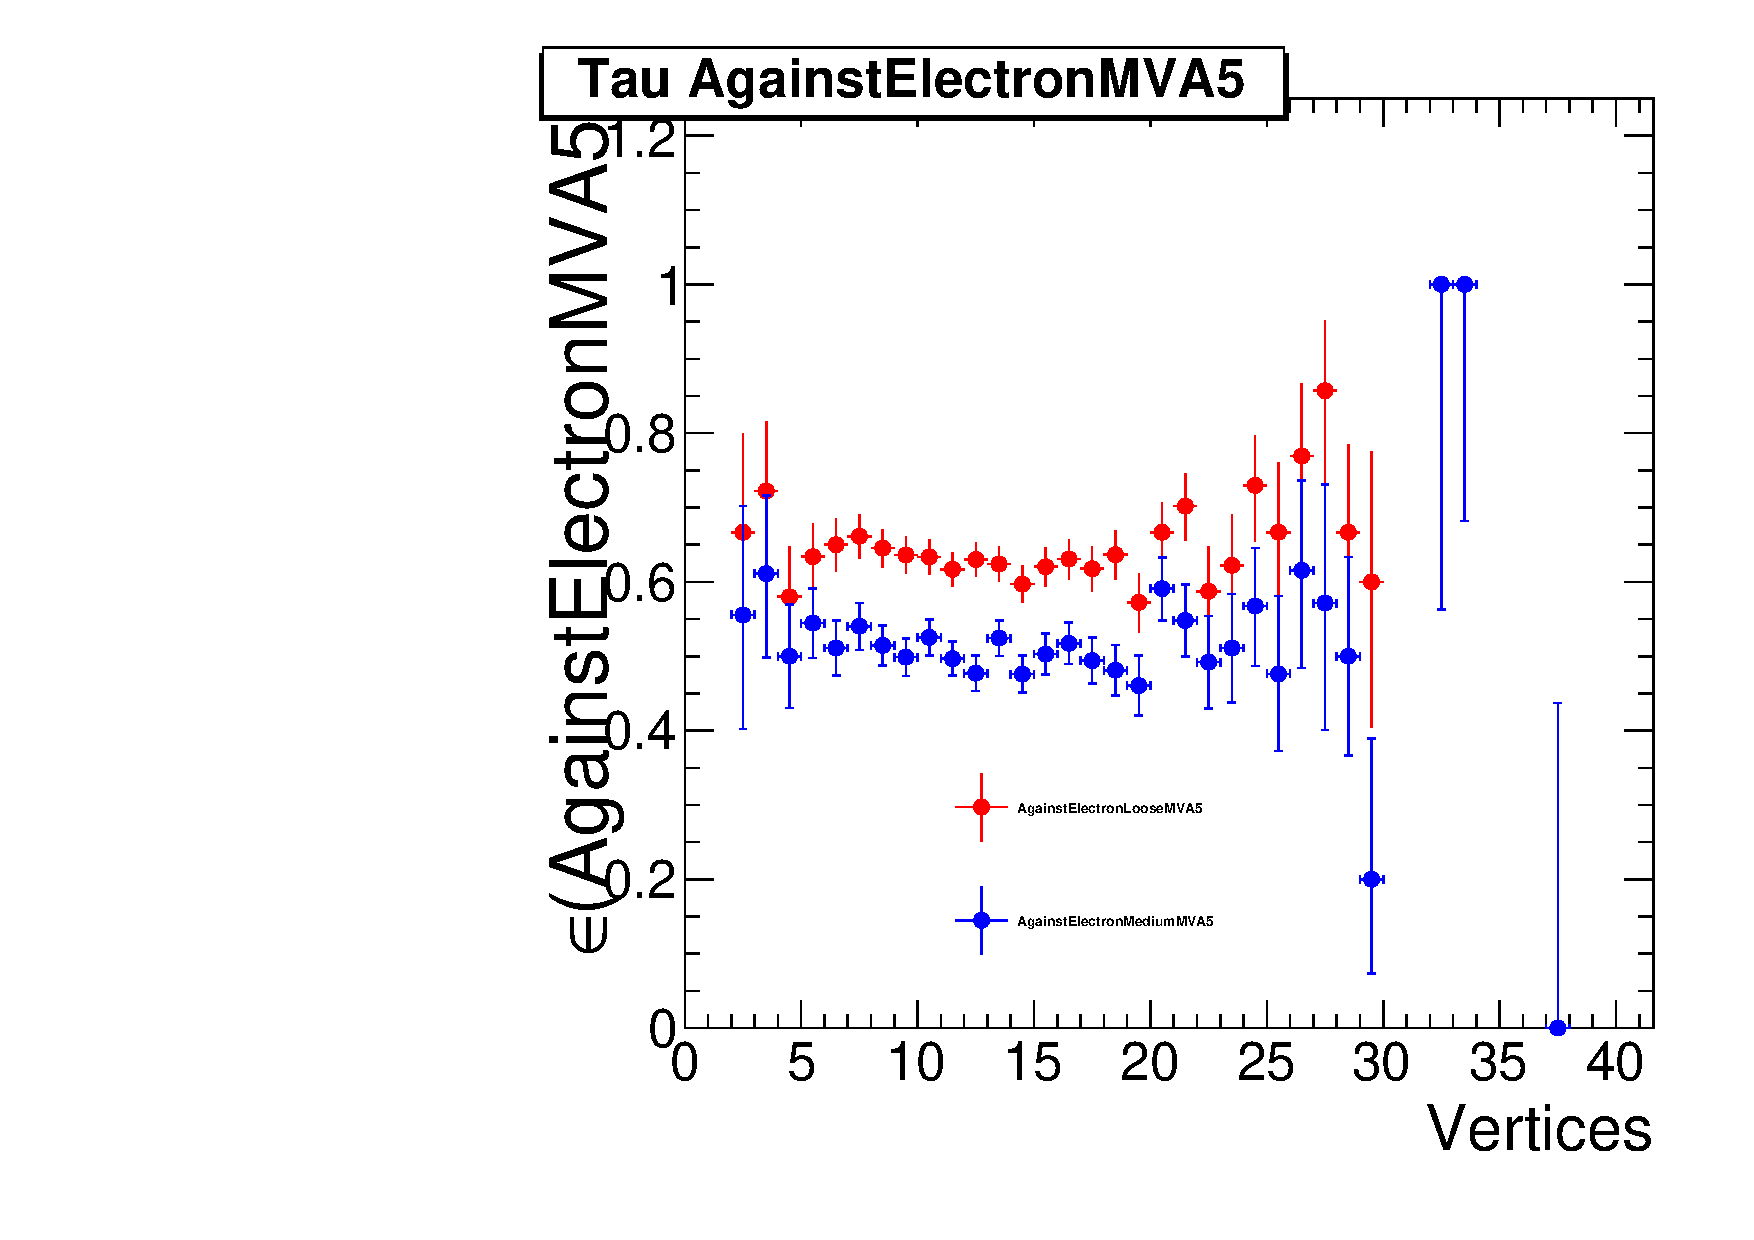
\includegraphics[width=0.50\textwidth]{figures/AgainstElectron_nvtx_4_29_16.pdf}
    \end{tabular}
    \caption{Efficiency of anti-electron discriminator (Loose/Medium MVA5) as function of $p_{T}$, $\eta$, and number of vertices of generator-level taus }
    \label{fig:EM5}
  \end{figure}

\begin{figure}[tbh!]
    \centering
    \begin{tabular}{cc}
      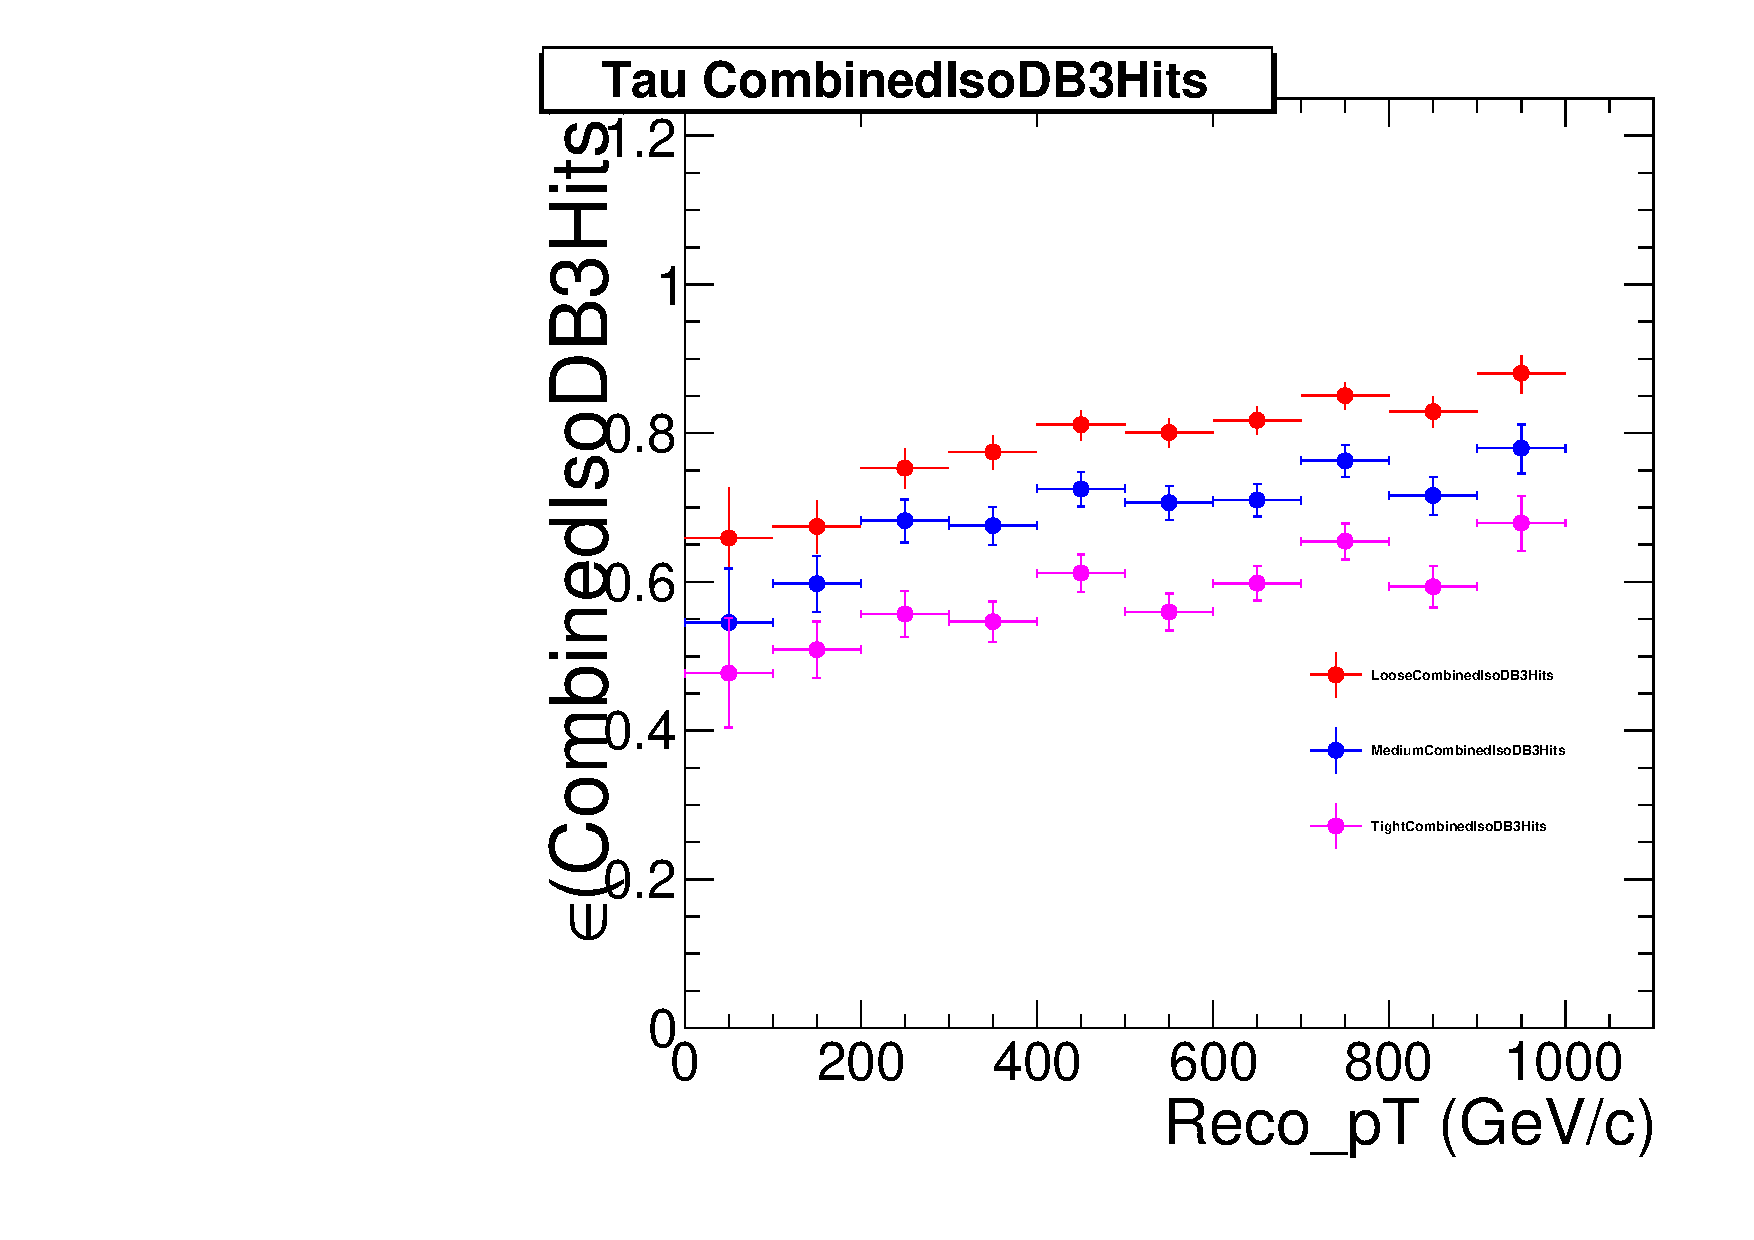
\includegraphics[width=0.50\textwidth]{figures/CombinedIso_4_29_16.pdf}
      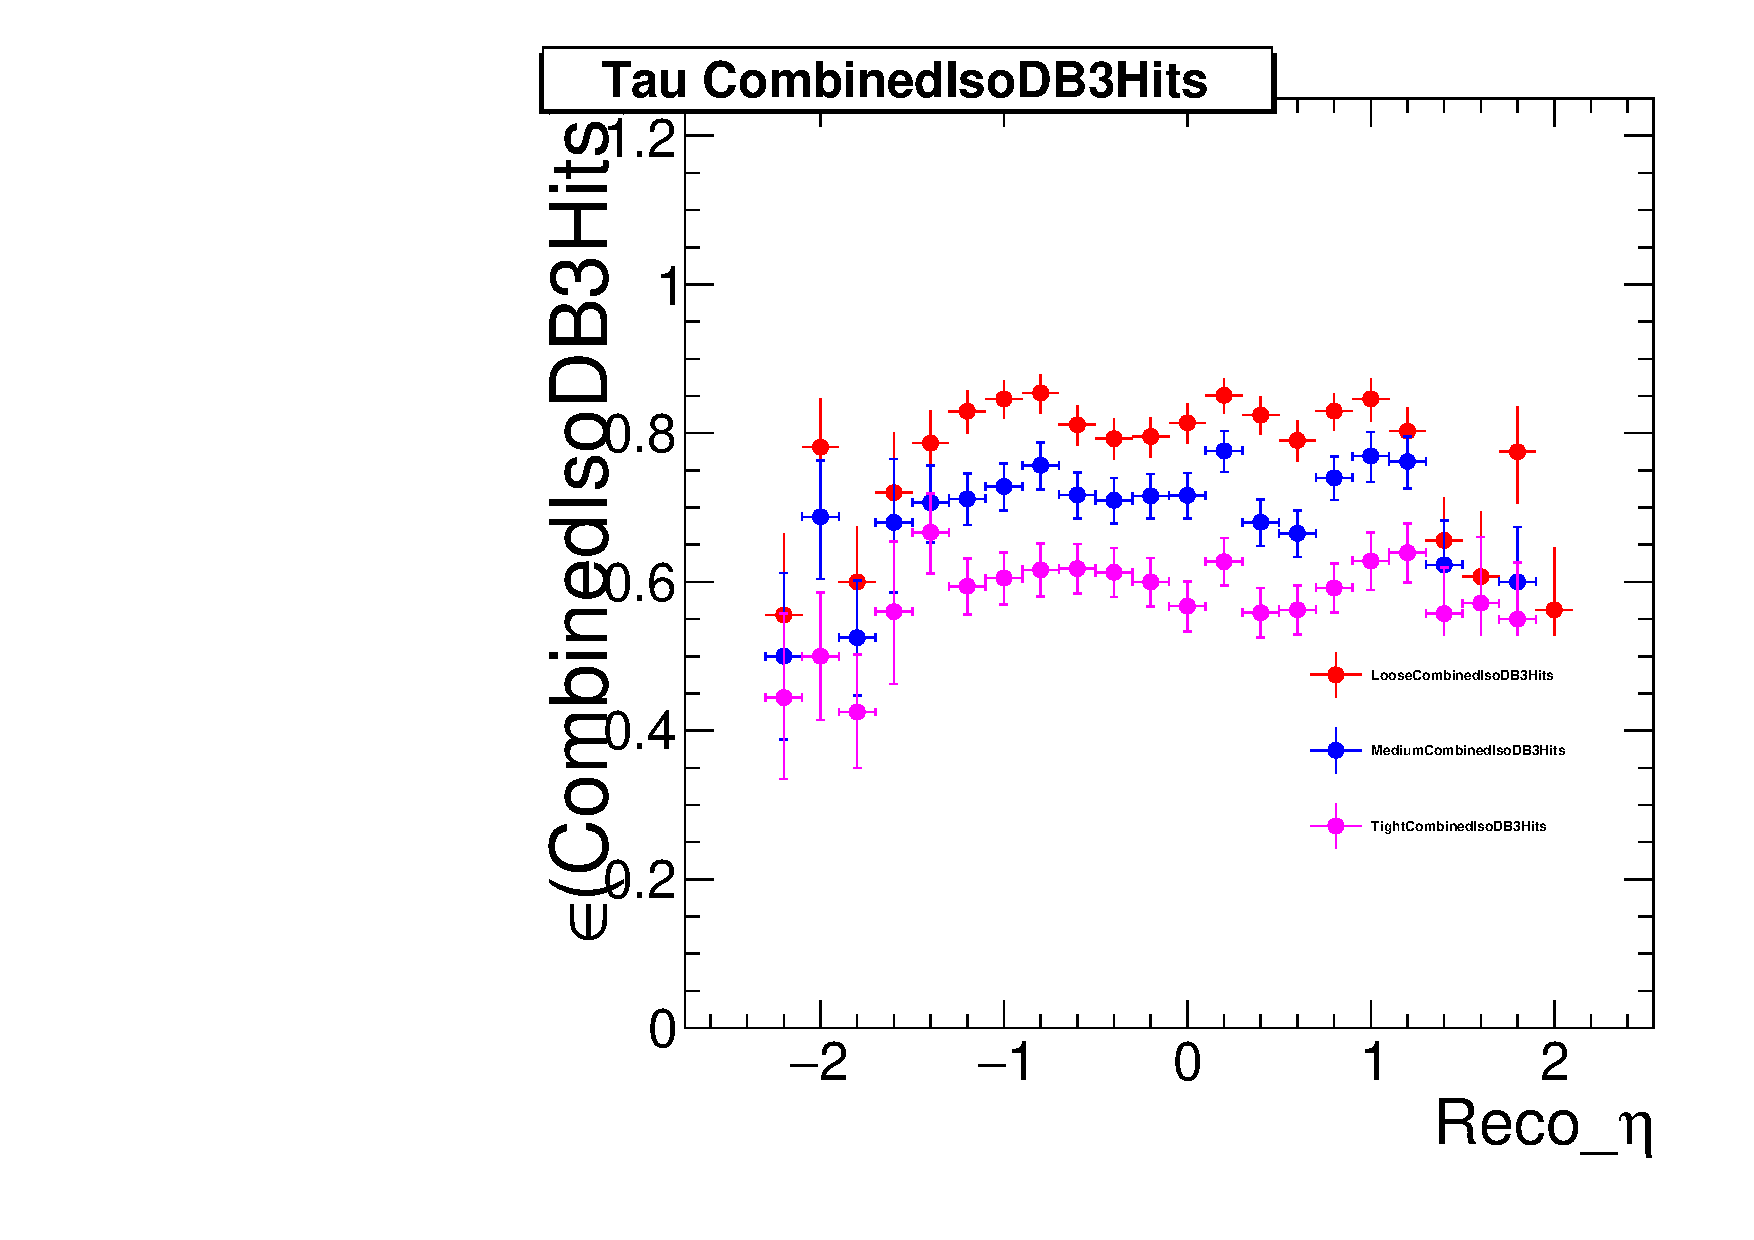
\includegraphics[width=0.50\textwidth]{figures/CombinedIso_eta_4_29_16.pdf}
       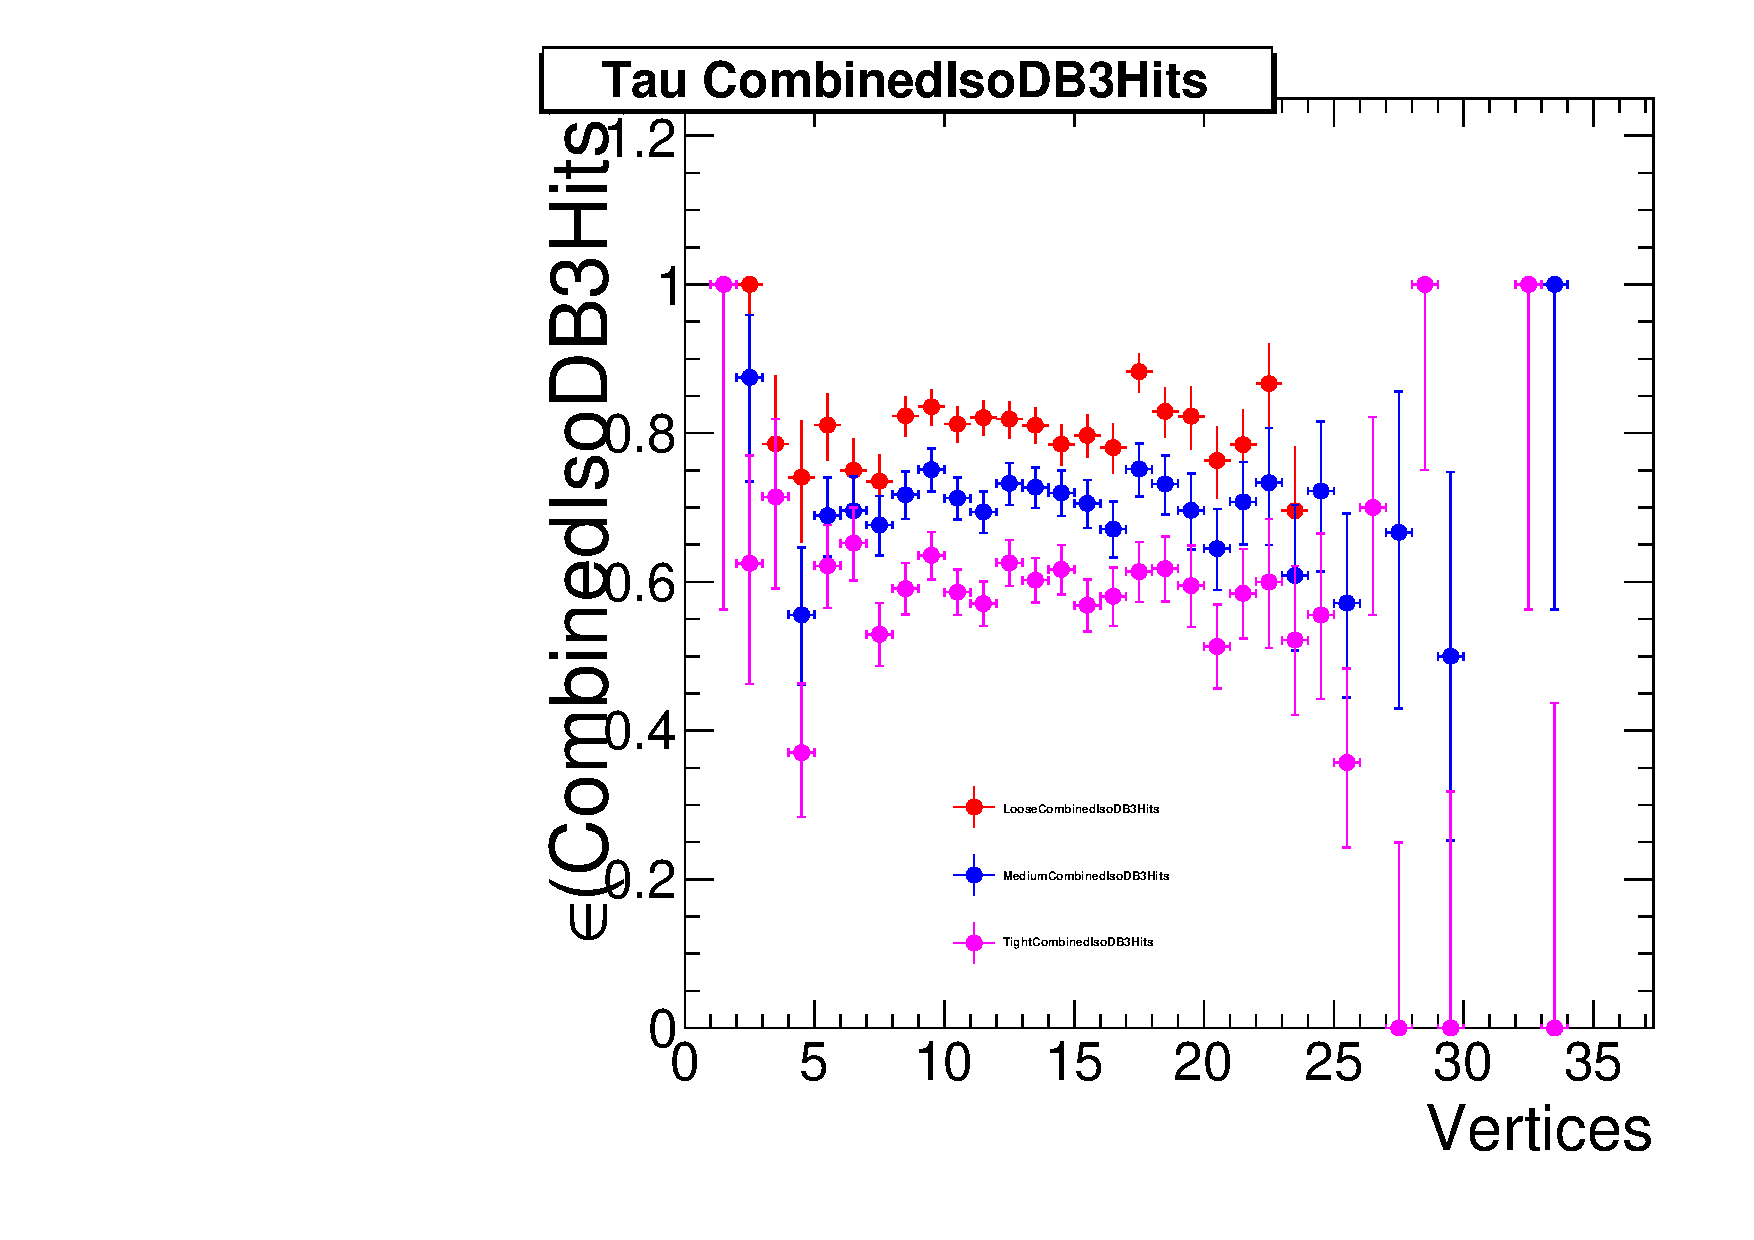
\includegraphics[width=0.50\textwidth]{figures/CombinedIso_nvtx_4_29_16.pdf}
    \end{tabular}
    \caption{Efficiency of isolation discriminator (``'CombinedIsoDB3Hits'') as function of $p_{T}$, $\eta$, and number of vertices of generator-level taus }
    \label{fig:TIso}
  \end{figure}



\subsubsection{Tau Energy Scale and Resolution}

Since the resolution and scale of our mass reconstruction depends on the effectiveness of the $\tau_{h}$ reconstruction, in this section we summarize our studies on $\tau_{h}$ response and resolution. We define the response as the difference between the transverse momentum of a reconstructed tau (that has passed all tau ID discriminators) and the transverse momentum of a generated tau that has been matched ($\Delta R < 0.3$) to the reconstructed tau. We can see from Figure \ref{fig:Tau2dResolution} (right) that the response distribution contains a narrow Gaussian-like component in the bulk, in addition to a relatively long tail (compared to electrons and muons). While the tails become less substantial at high $p_{T}$, the Gaussian-like bulk of the response distributions broaden at high $p_{T}$.
 
\begin{figure}[tbh!]
  \centering
  \begin{tabular}{cc}
  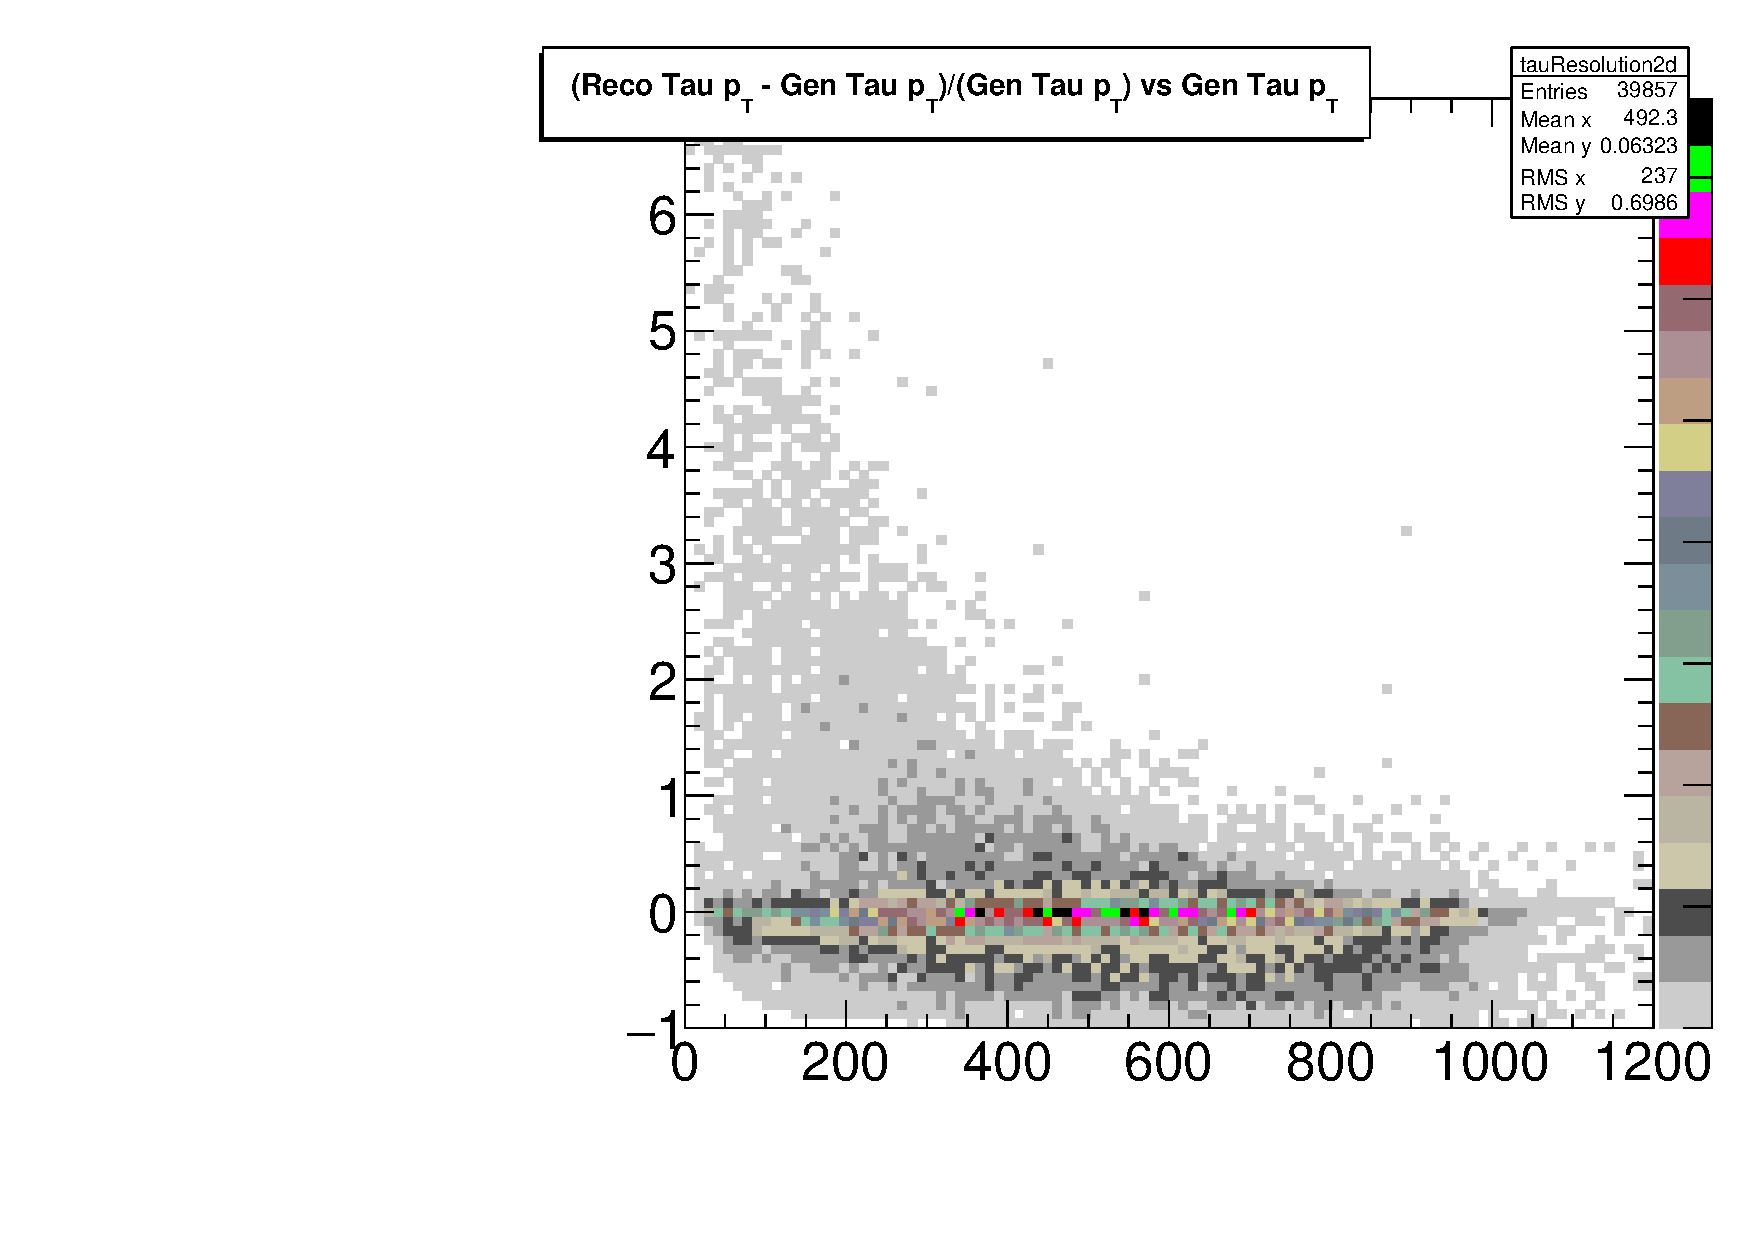
\includegraphics[width=0.50\textwidth]{figures/Tau2dResolution_4_29_16.pdf}
  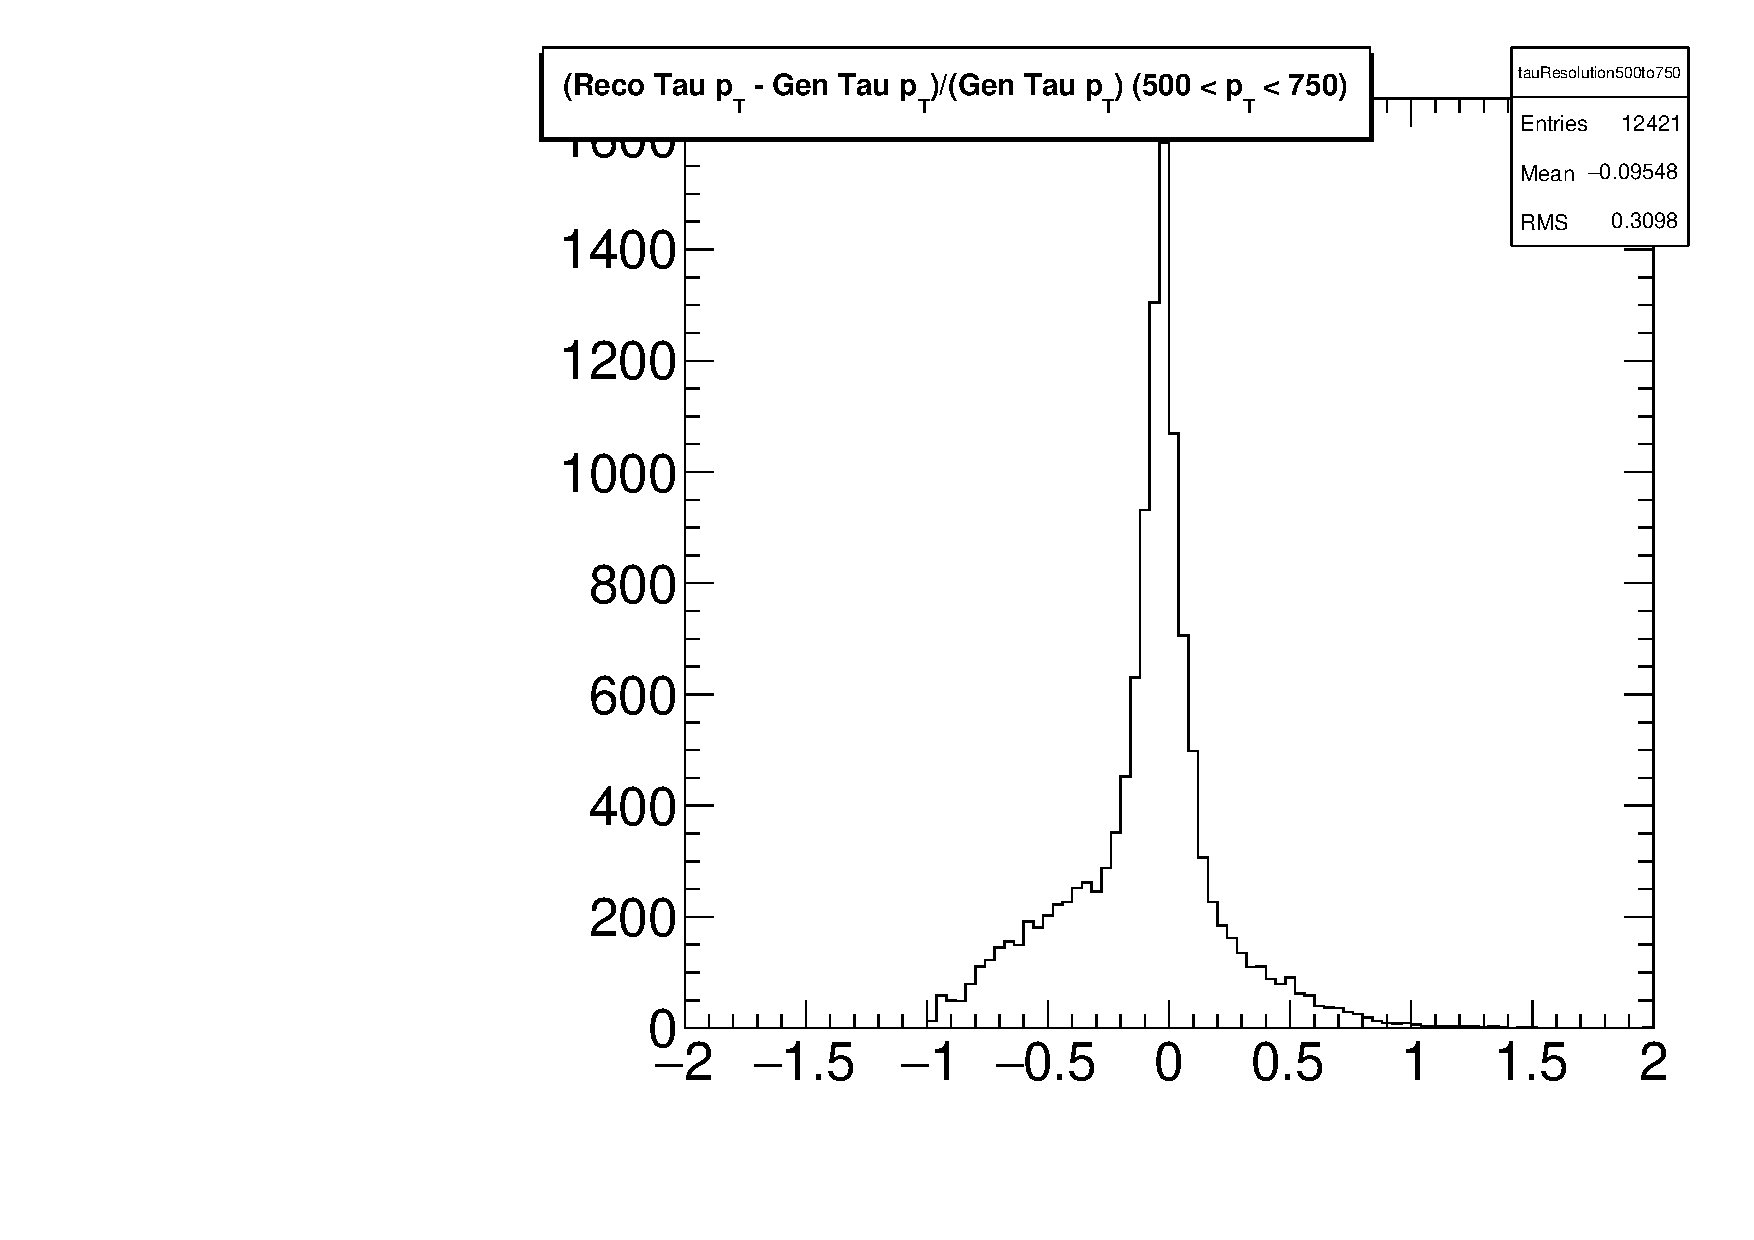
\includegraphics[width=0.50\textwidth]{figures/TauResolution_500to750_4_29_16.pdf}
  \end{tabular}
  \caption{Energy response of reconstructed taus, raw and vs. generated tau $p_{T}$}
  \label{fig:Tau2dResolution}
\end{figure}


%\begin{figure}[tbh!]
%    \centering
%    \begin{tabular}{cc}
%      \includegraphics[width=0.30\textwidth]{PLOTS/diTauPlots/Efficiency/comparison2GenTauPtFull.png}
%      \includegraphics[width=0.30\textwidth]{PLOTS/diTauPlots/Efficiency/comparison2GenTauEtaFull.png}
%       \includegraphics[width=0.30\textwidth]{PLOTS/diTauPlots/Efficiency/comparison2GenTauPhiFull.png}
%    \end{tabular}
%    \caption{Full TauID efficiency  as function of $p_{T}$ and $\eta$ , $\phi$ of generator-level taus }
%    \label{fig:Full}
%  \end{figure}
